%% elsarticle template — Expert Systems with Applications (Q1)
%% Role Specialization and Context Fragmentation in Multi-Agent LLM Systems
%% Author: Edurne Martínez de Contrasta | PROJENER.AI SL · UAX Campus Mare Nostrum 2026
%% VERSION v22 — Pre-submission changes: exploratory HDA limitations, 8B trade-off, Zenodo DOI

\documentclass[preprint,12pt,numrefs]{elsarticle}

\usepackage[utf8]{inputenc}
\usepackage[T1]{fontenc}
\usepackage[english]{babel}
\usepackage{textcomp}
\usepackage{amsmath,amssymb}
\usepackage{graphicx}
\usepackage{booktabs}
\usepackage{multirow}
\usepackage{array}
\usepackage{longtable}
\usepackage{tabularx}
\usepackage{xcolor}
\usepackage{hyperref}
\usepackage{xurl}
\usepackage{siunitx}
\usepackage{caption}
\usepackage{subcaption}
\usepackage{float}
\usepackage{enumitem}
\usepackage{listings}
\usepackage{tikz}
\usetikzlibrary{shapes.geometric,arrows.meta,positioning,babel}
\usepackage{lscape}
\sloppy
\setlength{\emergencystretch}{3em}
\lstset{
  basicstyle=\ttfamily\footnotesize,
  breaklines=true,
  breakatwhitespace=false,
  columns=flexible,
  linewidth=\columnwidth,
  xleftmargin=0pt,
  xrightmargin=0pt,
  frame=single,
  numbers=left,
  numberstyle=\tiny,
  keywordstyle=\color{blue},
  stringstyle=\color{red!60!black},
  commentstyle=\color{gray},
  showstringspaces=false
}

\journal{Expert Systems with Applications}

\begin{document}

\begin{frontmatter}

\title{Role Specialization and Context Fragmentation in Multi-Agent LLM
       Systems: An Empirical Study on Procurement Automation}

\author[uax,proj]{Edurne Martínez de Contrasta}

\address[uax]{Master's in Big Data and Business Analytics,
              Universidad Alfonso X el Sabio, Campus Mare Nostrum, Málaga, Spain}
\address[proj]{PROJENER.AI SL, Madrid, Spain}

\begin{abstract}
This paper investigates under what conditions multi-agent specialization
outperforms a single-agent approach in procurement automation, and when
the division into specialized roles generates context fragmentation that
prevents systemic risk detection. In the architectures we evaluate, each
agent perceives only a portion of the problem --- no single agent holds
a complete representation. Robotic Process Automation (RPA) systems handle
routine tasks well but fail on exceptions requiring reasoning, such as
contracts containing exclusivity clauses. Multi-agent systems based on
large language models (LLMs) emerge as a promising alternative in that
setting.

We propose a framework of five specialized agents orchestrated with
CrewAI. Nine variants were evaluated across 50~synthetic cases and
50~real cases drawn from the BPI Challenge~2019
\citep{vandongen2019bpi}. The Multi-Mixed variant (8B agents with a
70B decision-maker) achieved the highest Autonomous Resolution Rate
(ARR\,=\,98.7\,\%). The results provide empirical evidence consistent
with the compute equivalence hypothesis: a single agent with extended
context can match or exceed multi-agent performance under the same token
budget. That said, HDA --- an exploratory metric given the small 
number of positive cases ($n=13$) --- suggests that the most 
autonomous configurations may have limitations in detecting 
risks that require human intervention, though these differences 
lack statistical power to be conclusive.


Our primary contribution is an empirical analysis of the trade-offs
between autonomy and systemic risk detection under a controlled token
budget, including a role-level ablation study and validation on real
BPI Challenge 2019 data. The findings suggest that reliable risk
detection will likely require redesigning the information flows between
agents to mitigate context fragmentation --- rather than simply adding
more agents or scaling up model size.
\end{abstract}

\begin{keyword}
Multi-agent systems \sep
Large Language Models \sep
Procurement automation \sep
Human-in-the-Loop \sep
Compute equivalence \sep
Context fragmentation \sep
BPI Challenge 2019
\end{keyword}

\end{frontmatter}
%%------------------------------------------------------------------------------
\section{Introduction}
\label{sec:introduccion}

A technician needs to purchase a spare part. The supplier is approved,
budget is available, and the urgency is real. Yet the request will take
between three and seven days to receive a response, because it must pass
sequentially through the procurement, legal, finance, and compliance
departments. The administrative cost of processing that order is not
only financial --- it also includes the time burden placed on staff.

The problem is not bureaucracy itself, but that the systems designed to
automate it lack any capacity for reasoning. Robotic Process Automation
(RPA) systems execute repetitive, well-structured tasks efficiently.
They fail, however, when faced with regulatory deviations or conflicts
of interest. These systems do not reason, nor do they escalate
appropriately. They simply stop and wait for human intervention
\citep{Aguirre2017rpa}.

Multi-agent frameworks based on Large Language Models (LLMs) can go
beyond fixed rules: they can reason in the face of the unexpected.
Tools such as AutoGen \citep{wu2023autogen}, CrewAI \citep{crewai2024},
and LangGraph \citep{LangGraph2024} make it possible to build teams of
specialized agents capable of collaborating on exceptions. Work such as
ChatDev \citep{qian2023chatdev} showed that these teams can outperform
a single agent on complex tasks, while MetaGPT \citep{Hong2024metagpt}
and AgentVerse \citep{Chen2023agentverse} extended those results through
structured roles and inter-role coordination.

A question the literature has not yet answered well remains: when is it
actually worth using five agents instead of one? And when does
specialization become part of the problem rather than the solution?
Evidence in real enterprise environments is still sparse
\citep{Wang2024survey}. This work attempts to address that gap.

The main contributions of this study are: (i) a replicable multi-agent
framework across five business processes, together with evaluation data
and published source code; (ii) an empirical analysis of the
architectural trade-offs among \emph{compute equivalence}, model
diversity, and systemic risk detection; and (iii) a risk signal taxonomy
validated by six independent annotators ($\kappa$\,=\,0.652), which
helps explain why detection capacity varies substantially across domains.

The results suggest that multi-agent specialization introduces a
trade-off between autonomy and risk detection that cannot be resolved
simply by adding more agents or scaling up model size.

\paragraph{Research question}
\textit{Under what conditions does multi-agent specialization outperform
a single-agent approach in procurement process automation, and when does
context fragmentation impair systemic risk detection? Do these patterns
replicate on real-world data from the BPI Challenge~2019
\citep{vandongen2019bpi}?}

The paper is organized as follows: related work
(Sec.~\ref{sec:related}), framework (Sec.~\ref{sec:framework}),
experimental setup (Sec.~\ref{sec:setup}), results
(Sec.~\ref{sec:results}), comparative analysis
(Sec.~\ref{sec:comparative}), ablation study
(Sec.~\ref{sec:ablation}), cross-process and BPI validation
(Sec.~\ref{sec:crossprocess}), discussion
(Sec.~\ref{sec:discussion}), and conclusions
(Sec.~\ref{sec:conclusions}). The nine evaluated variants are
described in detail in Table~\ref{tab:variantes}
(Sec.~\ref{sec:framework}).
%%------------------------------------------------------------------------------
\section{Related Work}
\label{sec:related}

\subsection{Multi-Agent LLM Systems}

AutoGen \citep{wu2023autogen} introduced a multi-agent conversation
framework in which LLMs collaborate through structured messages.
CrewAI \citep{crewai2024} extends this paradigm with a role-and-task
model inspired by human organizations. Talebirad et al.\
\citep{talebirad2023} analyzed multi-agent collaboration as a mechanism
for amplifying the collective capacity of LLMs \citep{Wang2024survey}.
Park et al.\ \citep{park2023generative} documented emergent social
behaviors in agent communities. ChatDev \citep{qian2023chatdev} showed
that specialized agents can outperform a single agent on software
development tasks. MetaGPT \citep{Hong2024metagpt} assigned software
engineering roles to different agents and found that specialization
reduces hallucinations in code-related tasks. CAMEL \citep{Li2023camel}
proposed role-driven communication as a coordination mechanism --- a
direct antecedent of the design used here. AgentVerse
\citep{Chen2023agentverse} found that team composition affects
performance in a non-linear fashion. Li et al.\
\citep{Li2024moreagents} showed that scaling the number of agents
improves performance when the base model has sufficient capacity ---
a result consistent with the 8B--70B threshold identified in this work.

Modern LLMs combine chain-of-thought reasoning \citep{Wei2022cot} and
reactive acting \citep{Yao2023react}, which are the underlying cognitive
mechanisms of the specialized agents we evaluate. Factual hallucinations
\citep{Ji2023hallucination} represent the primary risk in enterprise
settings, which motivates the Human-in-the-Loop (HiL) mechanism
introduced in this work.

\subsection{Business Process Automation}

RPA systems --- UiPath \citep{UiPath2023} and Automation Anywhere
\citep{AutomationAnywhere2023} --- automate repetitive tasks well, but
their limitation is well documented: when an unforeseen exception
appears, they stop \citep{Aguirre2017rpa}. That is precisely what
motivates this work.

Benchmarks such as WorkArena \citep{drouin2024workarena} and TaskBench
\citep{lu2023taskbench} exist for evaluating agents in enterprise
environments, though neither targets procurement specifically with
annotated ground truth. ToolBench \citep{qin2023toolllm} and Toolformer
\citep{Schick2023toolformer} showed that LLMs can learn to use real APIs
autonomously, which supports the role-specific tool design used here.
APIBench \citep{patil2023gorilla} goes a step further by evaluating
whether LLMs generate correct API calls --- the same type of validation
we apply to the agents in this study.

Process mining \citep{VanDerAalst2011pm,VanDerAalst2012} provides the
methodological framework for analyzing processes from event logs. The
BPI Challenge~2019 \citep{vandongen2019bpi,VanDongen2011bpi} --- a
real-world Purchase-to-Pay event log with 251,734 cases --- serves as
the external validation benchmark for this work and as the source for
parametrizing the APIs with real statistics. The GDPR framework
\citep{GDPR2016} defines the regulatory requirements the Compliance
agent must verify, and the Human-in-the-Loop mechanism
\citep{Mosqueira2023hitl} ensures human oversight on the
highest-risk decisions.

\subsection{Compute Equivalence and Model Diversity}

Wu et al.\ \citep{wu2023autogen} argue that fair comparisons across
architectures should control for token budget, not just agent count.
We carry out that comparison empirically across three configurations:
Single-Small (200 tokens), Single-Small-XL (750 tokens), and
Multi-Small (750 tokens, 5 agents). If a single agent with more context
matches the multi-agent system, the architecture is not adding real
value. The experimental details are in Section~\ref{sec:comparative}.

The experiments use two models from the Llama~3 family
\citep{Meta2024llama3}: \texttt{llama-3.1-8b-instant} for the auxiliary
agents and \texttt{llama-3.3-70b-versatile} as the decision-maker in
the Mixed and Large variants. Both run via Groq \citep{Groq2024}, which
enables 70B-model inference with latencies below 3~seconds per case.
GPT-3 \citep{Brown2020gpt3} and GPT-4 \citep{OpenAI2023gpt4} are
included as state-of-the-art reasoning references, though they are not
used directly in the experiments.

In ensemble learning, mixing models of different sizes reduces error
correlation \citep{dietterich2000ensemble,Gomes2017ensemble}. That
principle is what we test by comparing Multi-Small (8B$\times$5),
Multi-Mixed (8B$\times$4+70B$\times$1), and Multi-Large (70B$\times$5).
The question is whether model diversity matters more than architecture.
Benchmarks such as SWE-bench \citep{Jimenez2024swebench} and GAIA
\citep{Mialon2023gaia} have set the standard for evaluating agents on
real tasks; we adapt that methodology here to the procurement domain
with our own ground truth.

Table~\ref{tab:related} positions this work relative to the most
relevant prior studies.

\begin{table}[htbp]
\centering
\caption{Comparison with related work. None of the prior studies
         evaluates the trade-off between multi-agent specialization
         and systemic risk detection on real process mining data.}
\label{tab:related}
\resizebox{\textwidth}{!}{%
\begin{tabular}{lllll}
\toprule
\textbf{Work} & \textbf{Architecture} & \textbf{Dataset} & \textbf{HDA} & \textbf{Gap} \\
\midrule
AutoGen \citep{wu2023autogen}         & Multi-agent  & Synthetic          & Not eval.\ & No risk detection \\
ChatDev \citep{qian2023chatdev}       & Multi-agent  & SWE-bench          & Not eval.\ & SW development only \\
AgentVerse \citep{Chen2023agentverse} & Multi-agent  & 204 tasks          & Not eval.\ & No real enterprise data \\
WorkArena \citep{drouin2024workarena} & Single-agent & ServiceNow         & Not eval.\ & No HiL mechanism \\
\textbf{This work}                    & Multi + Single & 50 synth.\ + BPI 2019 & Evaluated & Proc.\ + HiL + real data \\
\bottomrule
\end{tabular}%
}
\end{table}

%%------------------------------------------------------------------------------
\section{Proposed Framework}
\label{sec:framework}

\subsection{General Architecture}

The system is structured as a linear Directed Acyclic Graph (DAG) that
reflects how a procurement process actually works: budget is validated
first, then the contract is reviewed, and only at the end is the
compliance decision made. This ordering is not arbitrary --- it follows
real process dependencies. The orchestrator is CrewAI. In HiL variants,
the Compliance agent has explicit escalation rules that trigger whenever
it detects critical risk.

A graph with cycles would introduce circular dependencies that complicate
implementation without clear benefit in this domain (see
Table~\ref{tab:topologias} for a comparison of alternatives). This
architectural constraint --- the fixed DAG with no iteration --- is
documented in the Limitations section (Sec.~\ref{sec:limitations}) and
motivates the cross-process synthesis hypothesis.

\begin{table}[H]
\centering
\caption{Comparison of orchestration topologies for multi-agent
         procurement systems.}
\label{tab:topologias}
\resizebox{\textwidth}{!}{%
\begin{tabular}{llll}
\toprule
\textbf{Topology} & \textbf{Advantages} & \textbf{Limitations} & \textbf{Applicability} \\
\midrule
Linear DAG (CrewAI)        & Simple, predictable, easy to debug    & Context fragmentation, no iteration      & \checkmark\ Natural procurement flow \\
Graph with cycles           & Iterative feedback                    & Loop risk, higher latency                & $\times$\ Circular dependencies \\
Parallel processing         & Time efficiency                       & Synchronization complexity               & $\sim$\ Partially applicable \\
Adaptive graphs (LangGraph) & Dynamic conditional flows             & Higher implementation complexity         & $\sim$\ Future work \\
\bottomrule
\end{tabular}%
}
\end{table}

Analyzing the topology as an inter-agent communication network reveals
a notable bottleneck: the Finance agent acts as a structural bridge
between operational validation and regulatory decision-making. Its
betweenness centrality score is the highest in the system, meaning that
any information flowing from Procurement toward Legal passes necessarily
through it.
\medskip

The five agents and their main APIs are:
{\small
\begin{itemize}
  \item \textbf{Requester}: registers the request via
        \texttt{POST /api/requests/new}
  \item \textbf{Procurement}: validates the supplier via
        \texttt{GET /api/suppliers/\{id\}}
  \item \textbf{Finance}: verifies budget via
        \texttt{GET /api/budget/\{dept\}}
  \item \textbf{Legal}: analyzes contractual clauses via
        \texttt{POST /api/contracts/validate}
  \item \textbf{Compliance}: final decision-maker; escalates to a human via
        \texttt{POST /api/escalation/human} when critical risk is detected;
        queries the GDPR/CE/PRL/AESA regulatory database via
        \texttt{GET /api/regulations/\{cat\}}
\end{itemize}
}

The complete system prompts for each agent and the endpoint table are
included in Appendix~A and in the public repository.

\subsection{The Nine System Variants}

Table~\ref{tab:variantes} summarizes the configurations. Variants marked
with * report mean\,$\pm$\,$\sigma$ across three independent replications;
the rest are single runs.

\begin{table}[H]
\centering
\caption{Summary of variants and metrics. ARR: Autonomous Resolution Rate;
         HDA: HiL Detection Accuracy; DER: Decision Error Rate;
         PT: processing time per case (s). Variants marked * report
         mean\,$\pm$\,$\sigma$ (3~replications). Justification
         quality (SAT) reported in Appendix~E.}
\label{tab:variantes}
\resizebox{\textwidth}{!}{%
\begin{tabular}{llccccl}
\toprule
\textbf{Model} & \textbf{Config.} &
  \textbf{ARR} & \textbf{HDA} & \textbf{DER} &
  \textbf{PT} & \textbf{Purpose} \\
\midrule
RPA-Baseline*       & if-then rules                        & 100\%\,$\pm$\,0.0   & 0\%\,$\pm$\,0.0     & 34\%\,$\pm$\,0.0   & $\approx$0 & Minimum baseline \\
Single-Small*       & 8B\,$\times$1                        & 92\%\,$\pm$\,11.3   & 10.3\%\,$\pm$\,14.5 & 27.3\%\,$\pm$\,3.8 & 0.31       & LLM reference \\
Single-Small-XL*    & 8B\,$\times$1 (750~tok)              & 79.0\%\,$\pm$\,3.2  & 36.5\%\,$\pm$\,13.1 & 20.5\%\,$\pm$\,5.7 & 0.40       & Compute eq. \\
Multi-Small*        & 8B\,$\times$5                        & 79.5\%\,$\pm$\,7.1  & 21.2\%\,$\pm$\,10.6 & 27.8\%\,$\pm$\,4.7 & 1.74       & Main multi \\
Multi-Small-Abl     & 8B\,$\times$3                        & 88\%                & 0\%                 & 30\%               & 0.77       & Ablation \\
Multi-Mixed*        & 8B\,$\times$4+70B\,$\times$1         & 98.7\%\,$\pm$\,0.9  & 5.1\%\,$\pm$\,3.6   & 27.3\%\,$\pm$\,0.9 & 1.69       & Best ARR/cost \\
Multi-Large         & 70B\,$\times$5                       & 98\%                & 0\%                 & 26\%               & 2.40       & Homog.\ powerful \\
Multi-Mixed-HiL     & 8B\,$\times$4+70B\,$\times$1+HiL    & 98\%                & 0\%                 & 28\%               & 1.56       & Active HiL \\
Multi-Mixed-HiL-Clf & 2-stage, 8B                          & 94\%                & 23.1\%              & 22\%               & 2.85       & Best dep.\ HDA \\
\midrule
\textit{AutoGen 0.7.5} & \textit{RoundRobin, 8B$\times$5} & \textit{100\%} & \textit{0\%} & \textit{76\%} & \textit{6.55} & \textit{Alt.\ baseline} \\
\bottomrule
\end{tabular}%
}
\end{table}

%%------------------------------------------------------------------------------
\section{Experimental Setup}
\label{sec:setup}

\subsection{Dataset and Metrics}

We designed 50 procurement cases with annotated ground truth at three
levels: \emph{Simple} (C01--C20, standard purchases), \emph{Medium}
(C21--C38, operational exceptions), and \emph{Complex} (C39--C50,
regulatory and strategic exceptions).

Of the 50 cases, 13 require HiL escalation. The distribution follows
the methodology of WorkArena \citep{drouin2024workarena} and AgentBench
\citep{liu2023agentbench} for controlled environments with annotated
ground truth. Evaluation on real data was carried out on the BPI
Challenge~2019 \citep{vandongen2019bpi}
(Sec.~\ref{sec:crossprocess}).

The main metrics are ARR (\emph{Autonomous Resolution Rate}, target
$>70$\%, consistent with WorkArena \citep{drouin2024workarena} benchmarks
for enterprise task automation), HDA (\emph{HiL Detection Accuracy},
reported as an exploratory metric given the small number of positive
cases, $n=13$; target $>90$\% reflects the safety requirement that
critical risk cases should rarely go undetected in regulated
procurement), DER (\emph{Decision Error Rate}, target $<10$\%,
aligned with acceptable error rates in automated business process
systems \citep{Aguirre2017rpa}), and PT (\emph{Process Time}).
SAT (\emph{Satisfaction Score}) is evaluated by LLM-as-Judge
\citep{zheng2023judging} on clarity, completeness, and actionability
(1--5 scale, target $>3{.}5$); note that this metric has not been
validated against human evaluators and should be treated as
indicative only.

\subsection{Technology Stack and Reproducibility}

\begin{itemize}
  \item Framework: CrewAI, Python~3.12, Windows~10, Jupyter~Lab
  \item Auxiliary LLM: \texttt{llama-3.1-8b-instant} via Groq~API \citep{Groq2024}
  \item Decision LLM (Mixed/Large): \texttt{llama-3.3-70b-versatile} via Groq~API
  \item Temperature: 0.0 (with the caveat documented below)
  \item Anti-rate-limit pause: 4--8~s between cases depending on model
  \item Code: \url{https://github.com/Edurne0781/multiagent-procurement-llm}
\end{itemize}

A clarification on determinism is warranted. The \texttt{temperature=0.0}
setting was verified in a single session: five test cases produced
identical outputs. The robustness analysis across three independent
replications (Table~\ref{tab:replicas}), however, shows
$\sigma$\,ARR\,=\,11.3\,pp for the 8B model --- consistent with the
literature on non-determinism in distributed LLM inference
\citep{ouyang2023nondeterminism}. Groq introduces variability even at
fixed temperature due to differences in server state and dynamic
batching. Multi-Mixed ($\sigma$\,=\,0.9\,pp) is considerably more
stable and offers the best ARR/stability balance among the evaluated
configurations, though its exploratory HDA limits its applicability in
settings with strict risk detection requirements.
%%------------------------------------------------------------------------------
\section{Results}
\label{sec:results}

\subsection{Overview}

Figure~\ref{fig:metricas_principales} shows the three main metrics.
Table~\ref{tab:variantes} reports the complete values with standard
deviations.

\begin{figure}[H]
  \centering
  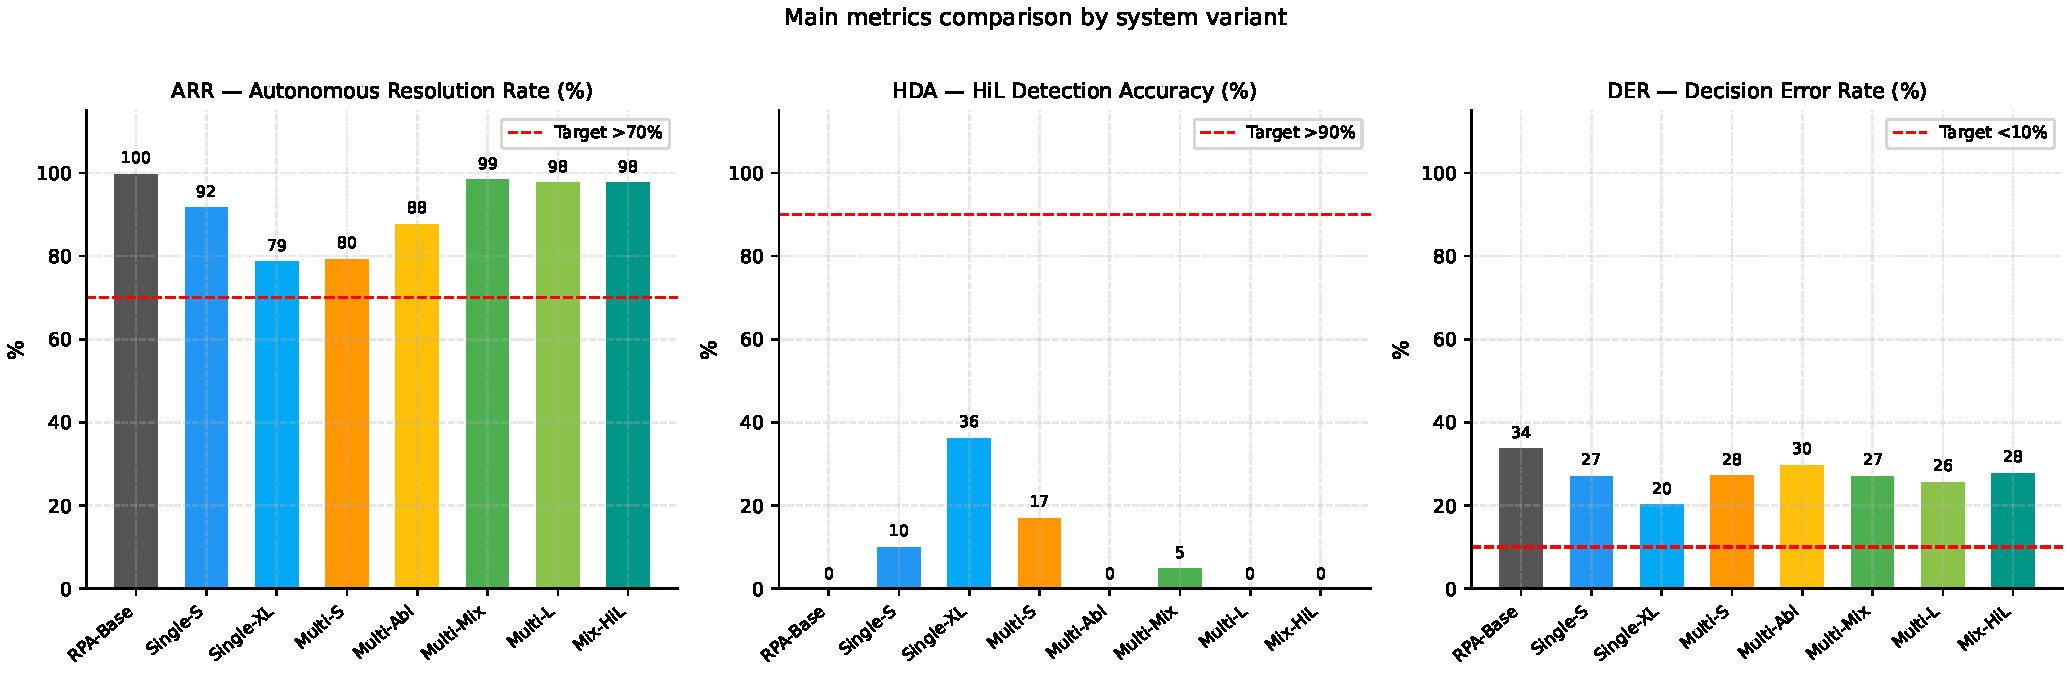
\includegraphics[width=\textwidth,height=0.42\textheight,keepaspectratio]{figura1}
  \caption{Comparison of ARR, HDA, and DER. Left: Autonomous Resolution
           Rate (target $>70$\%). Center: HiL Detection Accuracy
           (exploratory metric, $n=13$ positive cases). Right: Decision
           Error Rate (target $<10$\%).}
  \label{fig:metricas_principales}
\end{figure}

The most notable findings: Multi-Mixed achieves the highest ARR (98.7\%)
with minimal variability, but its HDA is very low (5.1\%). Single-Small,
using a smaller model, reaches HDA\,=\,10.3\% on average (30.8\% in the
first replication). Single-Small-XL and Multi-Small converge to nearly
identical ARR means (79.0\% vs.\ 79.5\%) over four replications,
consistent with the compute equivalence hypothesis. The RPA-Baseline
delivers exactly what one would expect: ARR\,=\,100\% because it never
escalates, HDA\,=\,0\%, DER\,=\,34\%.

\begin{table}[htbp]
\centering
\caption{Results by replication. The variability of Single-Small
         ($\sigma$\,ARR\,=\,11.3\,pp) contrasts with the stability of
         Multi-Mixed when the decision-maker is the 70B model
         ($\sigma$\,=\,0.9\,pp). Single-Small-XL and Multi-Small
         were run over four replications to verify the compute
         equivalence hypothesis under the high variance of the 8B
         model; the remaining variants were replicated three times.
         {---} indicates no fourth replication was conducted.}
\label{tab:replicas}
\begin{tabular}{lccccc}
\toprule
\textbf{Model} & \textbf{Rep.\ 1} & \textbf{Rep.\ 2} & \textbf{Rep.\ 3} &
  \textbf{Rep.\ 4} & \textbf{Mean\,$\pm$\,$\sigma$} \\
\midrule
RPA-Baseline ARR & 100\% & 100\% & 100\% & --- & 100\%\,$\pm$\,0.0\,pp \\
RPA-Baseline HDA & 0\%   & 0\%   & 0\%   & --- & 0\%\,$\pm$\,0.0\,pp   \\
\midrule
Single-Small ARR & 76\%   & 100\% & 100\% & --- & 92\%\,$\pm$\,11.3\,pp \\
Single-Small HDA & 30.8\% & 0\%   & 0\%   & --- & 10.3\%\,$\pm$\,14.5\,pp \\
Single-Small DER & 22\%   & 28\%  & 32\%  & --- & 27.3\%\,$\pm$\,3.8\,pp  \\
\midrule
Single-Small-XL ARR & 84\% & 76\% & 76\% & 80\% & 79.0\%\,$\pm$\,3.2\,pp \\
Single-Small-XL HDA & 23.1\% & 53.8\% & 30.8\% & 53.8\% & 40.4\%\,$\pm$\,13.1\,pp \\
Single-Small-XL DER & 28\% & 24\% & 14\% & 16\% & 20.5\%\,$\pm$\,5.7\,pp \\
\midrule
Multi-Small ARR & 68\% & 82\% & 80\% & 88\% & 79.5\%\,$\pm$\,7.1\,pp \\
Multi-Small HDA & 30.8\% & 7.7\% & 15.4\% & 15.4\% & 17.3\%\,$\pm$\,8.5\,pp \\
Multi-Small DER & 28\% & 30\% & 26\% & 26\% & 27.5\%\,$\pm$\,1.6\,pp \\
\midrule
Multi-Mixed ARR  & 100\%  & 98\%  & 98\%  & --- & 98.7\%\,$\pm$\,0.9\,pp \\
Multi-Mixed HDA  & 0\%    & 7.7\% & 7.7\% & --- & 5.1\%\,$\pm$\,3.6\,pp  \\
Multi-Mixed DER  & 26\%   & 28\%  & 28\%  & --- & 27.3\%\,$\pm$\,0.9\,pp \\
\bottomrule
\end{tabular}
\end{table}

The table shows that the ARR difference between Single-Small and
Multi-Mixed is not statistically distinguishable when comparing
replication means --- the 6.7\,pp gap falls within Single-Small's
standard error. The case-level McNemar test (Table~9) does reach
significance, but addresses a different question: item-level agreement,
not architectural stability. What the replication analysis makes clear
is the stability difference: $\sigma = 0.9$\,pp vs.\ $11.3$\,pp.

Single-Small-XL and Multi-Small were run over four replications
to verify the compute equivalence hypothesis under the high variance
of the 8B model ($\sigma$\,=\,11.3\,pp). Their means converge to
nearly identical values (79.0\%\,$\pm$\,3.2\,pp vs.\
79.5\%\,$\pm$\,7.1\,pp), which confirms that with
\texttt{llama-3.1-8b-instant} neither expanding the context window
nor adding specialized agents produces a consistent advantage. The
remaining variants were replicated three times, consistent with
standard practice for non-deterministic LLM evaluation
\citep{ouyang2023nondeterminism}.


\begin{table}[H]
\centering
\caption{Confusion matrix for the 13 HiL cases ($n=13$,
         \textit{requires\_hil}=True). TP: true positive (correctly
         escalated); TN: true negative; FP: false alarm; FN: undetected
         risk case.}
\label{tab:confusion_hil}
\begin{tabular}{lcccc}
\toprule
\textbf{Variant} & \textbf{TP} & \textbf{TN} & \textbf{FP} & \textbf{FN} \\
\midrule
Single-Small        & 4 & 29 & 8 & 9 \\
Multi-Mixed         & 0 & 37 & 0 & 13 \\
Multi-Mixed-HiL-Clf & 3 & 37 & 0 & 10 \\
\bottomrule
\end{tabular}
\end{table}

Multi-Mixed produces no false alarms (FP\,=\,0) but also detects no
real risk cases (FN\,=\,13). Multi-Mixed-HiL-Clf is the only
deployable variant with perfect precision on the cases it escalates
(0 false positives), though its recall remains low (3 out of 13).

\subsection{Per-Variant Analysis}

\emph{Note: values in this subsection correspond to the initial single
run. Summary statistics (mean\,$\pm$\,$\sigma$ across 3~replications)
are in Table~\ref{tab:replicas}.}
\paragraph{RPA-Baseline}
ARR\,=\,100\% because it never escalates --- it approves or rejects
mechanically. HDA\,=\,0\%, DER\,=\,34\% (1 in every 3 decisions is
wrong). In case C24, the RPA approves a contract containing an
exclusivity clause because the supplier is registered and budget is
available, without evaluating the legal risk. This is the lower bound
of the experiment: any LLM-based system must improve on this DER.
\paragraph{Single-Small (8B, 200~tok)}
ARR\,=\,76\%, HDA\,=\,30.8\%, DER\,=\,22\%. Most token- and
time-efficient (PT\,=\,0.31\,s). Inter-replication variability is high
($\sigma$\,=\,11.3\,pp in ARR): in replications~2 and~3, HDA drops to
0\%, which limits the interpretability of that value.
\paragraph{Multi-Small (8B$\times$5)}
ARR\,=\,79.5\%\,$\pm$\,7.1\,pp (mean over 4~replications), virtually
indistinguishable from Single-Small-XL (79.0\%\,$\pm$\,3.2\,pp) at the
same token budget. The first replication gave 68\%, but subsequent runs
showed higher variance, consistent with the non-deterministic behaviour
of \texttt{llama-3.1-8b-instant} on distributed inference. Multi-agent
architecture provides no consistent advantage with small models.
\paragraph{Multi-Mixed (8B$\times$4 + 70B$\times$1)}
ARR\,=\,98.7\%\,$\pm$\,0.9\,pp, the largest jump in the experiment
(+19.2\,pp over Multi-Small mean). The Compliance decision-maker uses
the 70B model. DER\,=\,27.3\%, estimated cost \$0.0065/case. This is
the most stable configuration in the experiment.
\paragraph{Multi-Large (70B$\times$5)}
ARR\,=\,98\%, virtually identical to Multi-Mixed despite using powerful
models throughout. It costs 2.7$\times$ more for comparable results,
which is consistent with the bottleneck in Multi-Mixed having been the
decision-maker rather than the auxiliary agents.
\paragraph{Multi-Mixed-HiL-Clf}
ARR\,=\,94\%, HDA\,=\,23.1\%, DER\,=\,22\%, PT\,=\,2.85\,s. Best
deployable variant in terms of HDA. The 3~escalated cases match the
ground truth \texttt{requires\_hil=True} exactly, with 0~false
positives.

\begin{table}[H]
\centering
\caption{95\% confidence intervals for ARR and HDA. The high
         variability of Single-Small means its ARR difference from
         Multi-Mixed is not statistically distinguishable, though
         Multi-Mixed is substantially more stable.}
\label{tab:ic}
\begin{tabular}{lcccc}
\toprule
\textbf{Model} & \textbf{ARR (\%)} & \textbf{95\% CI ARR} &
  \textbf{HDA (\%)} & \textbf{95\% CI HDA} \\
\midrule
RPA-Baseline  & $100.0 \pm 0.0$  & [100.0, 100.0]  & $0.0 \pm 0.0$   & [0.0, 0.0] \\
Single-Small  & $92.0 \pm 11.3$  & [69.0, 115.0]$^\dagger$ & $10.3 \pm 14.5$ & [0, 39.3] \\
Multi-Mixed   & $98.7 \pm 0.9$   & [96.9, 100.5]   & $5.1 \pm 3.6$   & [1.5, 8.7] \\
\bottomrule
\end{tabular}
\par\smallskip
\footnotesize $^\dagger$CI truncated to valid range [0, 100].
\end{table}


\subsection{Sensitivity Analysis and Confidence Intervals}

The ARR difference between Single-Small and Multi-Mixed (6.7\,pp) is
smaller than the standard error of Single-Small (11.3\,pp), so it is
not statistically significant in ARR terms. What differs substantially
is stability: $\sigma$\,=\,0.9\,pp vs.\ 11.3\,pp.

\subsection{Computational Cost and Efficiency Frontier}

\begin{table}[H]
\centering
\caption{Token consumption and estimated cost per model. Costs are
         estimated at GPT-3.5-turbo market prices for comparability;
         in production with free-tier Groq, the actual cost is \$0.00.}
\label{tab:tokens}
\resizebox{\textwidth}{!}{%
\begin{tabular}{lrrrrl}
\toprule
\textbf{Model} & \textbf{Tok/case} & \textbf{Total tok} &
  \textbf{Calls} & \textbf{Cost (\$)} & \textbf{Note} \\
\midrule
RPA-Baseline        &   0 &      0 & 0 & \$0.0000 & No LLM \\
Single-Small        & 200 & 10{,}000 & 1 & \$0.0012 & Most token-efficient \\
Single-Small-XL     & 750 & 37{,}500 & 1 & \$0.0045 & Compute eq.\ confirmed (4 reps.) \\
Multi-Small         & 750 & 37{,}500 & 5 & \$0.0045 & Indistinguishable from XL \\
Multi-Small-Abl     & 450 & 22{,}500 & 3 & \$0.0027 & 40\% saving vs.\ Multi-Small \\
Multi-Mixed         & 750 & 37{,}500 & 5 & \$0.0065 & Optimal cost/performance \\
Multi-Large         & 750 & 37{,}500 & 5 & \$0.0120 & 2.7$\times$ Multi-Mixed, same ARR \\
Multi-Mixed-HiL     & 875 & 43{,}750 & 5 & \$0.0053 & Balanced ARR/cost \\
\bottomrule
\end{tabular}%
}
\end{table}

\subsection{Justification Quality: LLM-as-Judge}

Multi-Mixed produces the highest-quality justifications
(SAT\,=\,4.36) and the most consistent ones ($\sigma$\,=\,0.27, the
lowest across all variants). RPA-Baseline falls below the minimum
threshold: justifications of the type ``Supplier OK + budget OK''
give the recipient no guidance on what to do
(actionability\,=\,2.40).

Full results are reported in Appendix~\hyperref[app:sat]{E}.

\begin{figure}[H]
  \centering
  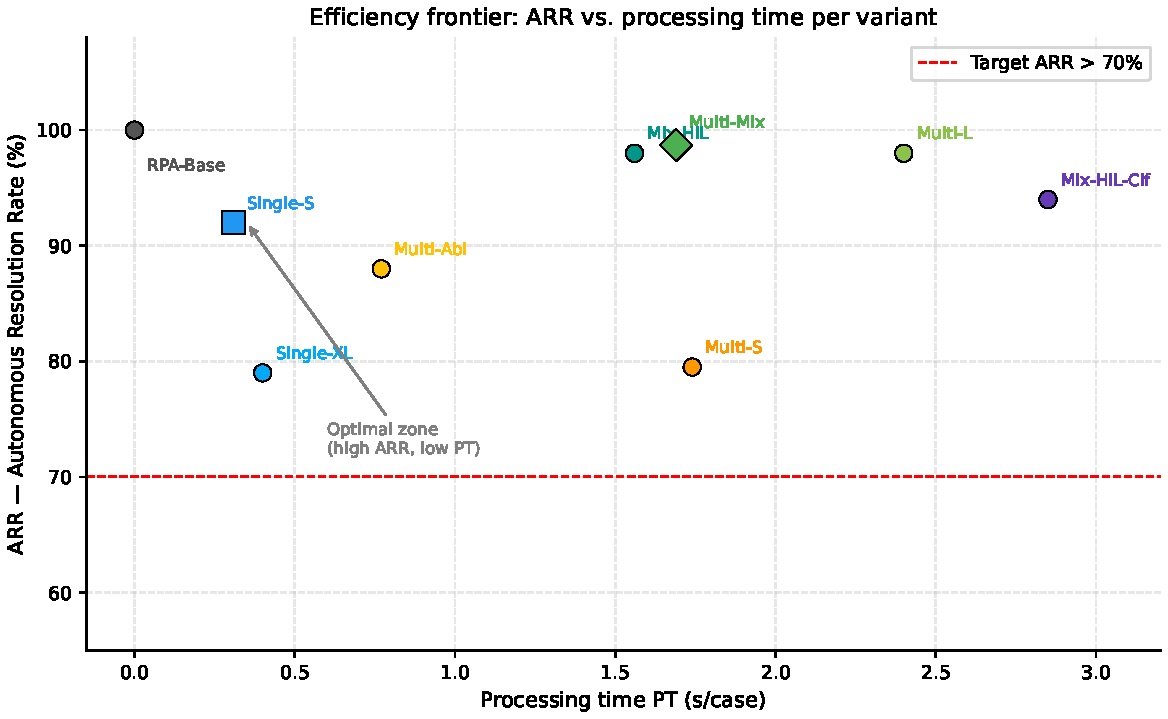
\includegraphics[width=0.85\textwidth,height=0.38\textheight,keepaspectratio]{figura2}
  \caption{Efficiency frontier: ARR vs.\ processing time per case.
           Single-Small offers the best ARR/efficiency balance for
           lightweight deployments; Multi-Mixed reaches optimal ARR
           at moderate processing time.}
  \label{fig:eficiencia}
\end{figure}

Single-Small stands out as the most efficient option for lightweight
deployments: it resolves 76\% of cases in 0.31~seconds per case.
Multi-Mixed reaches the highest ARR but requires 1.69~seconds --- a
reasonable time for enterprise settings where accuracy matters more
than speed.

\begin{figure}[H]
  \centering
  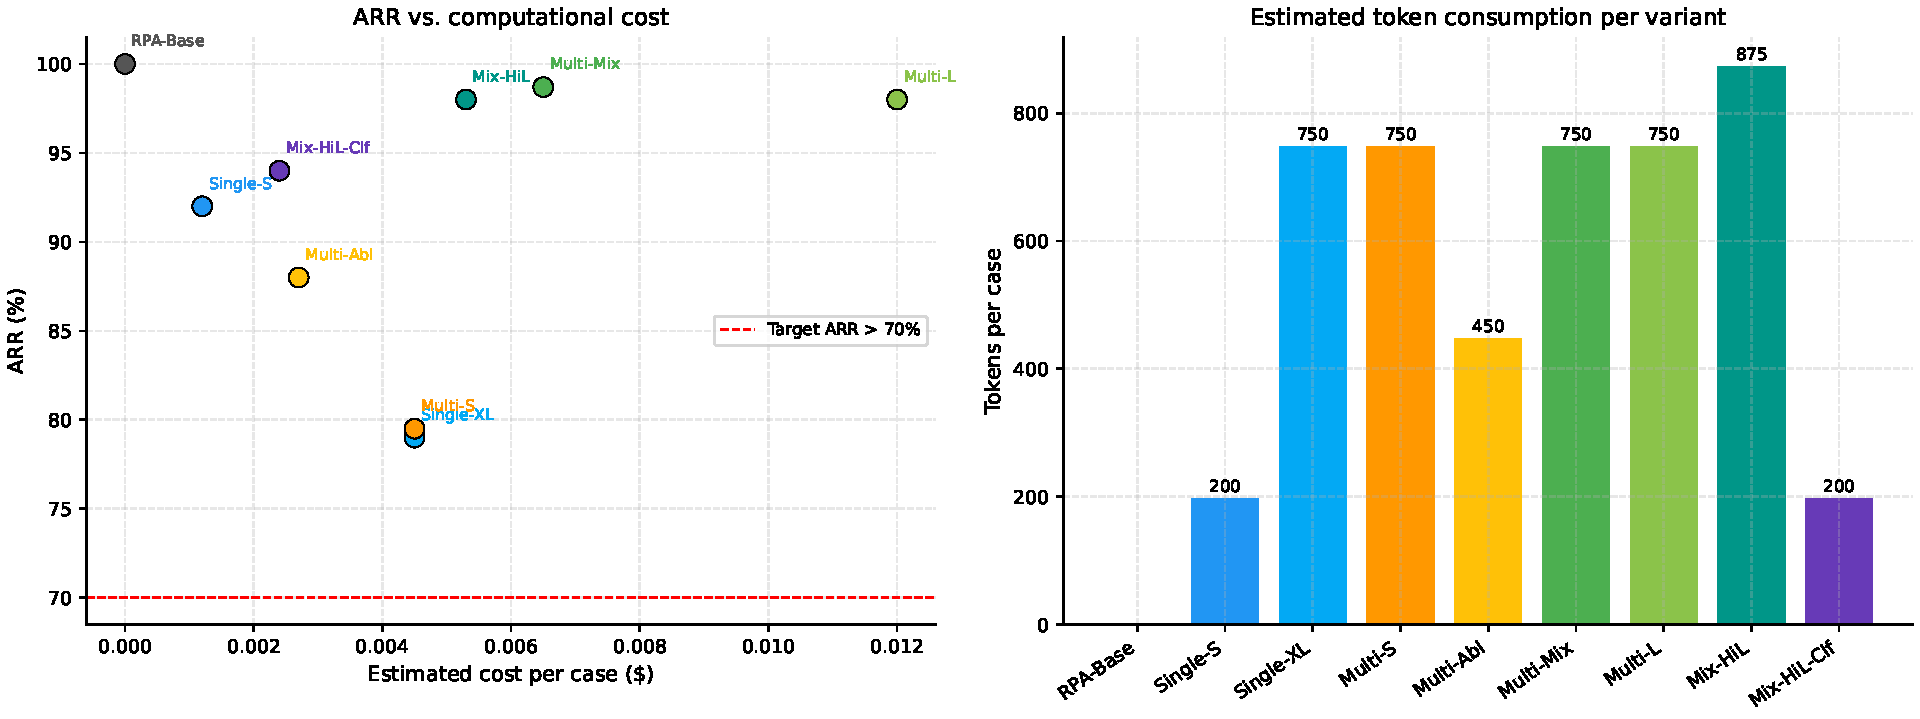
\includegraphics[width=0.85\textwidth,height=0.38\textheight,keepaspectratio]{figura5}
  \caption{ARR vs.\ token cost (left) and estimated token consumption
           per model (right). Multi-Mixed is the optimal cost/performance
           point.}
  \label{fig:coste}
\end{figure}



\begin{table}[H]
\centering
\caption{McNemar test with continuity correction on the ARR criterion
         ($n=37$ non-HiL cases). Significance: *\,$p<0.05$,
         **\,$p<0.01$, n.s.\ not significant.}
\label{tab:mcnemar}
\begin{tabular}{lrrrrl}
\toprule
\textbf{Comparison} & \textbf{ARR\,A} & \textbf{ARR\,B} &
  $\boldsymbol{b}$ & $\boldsymbol{c}$ & \textbf{Sig.} \\
\midrule
RPA-Baseline vs.\ Single-Small   & 100.0\% & 78.4\%  & 8 & 0 & * \\
Single-Small vs.\ Multi-Mixed    &  78.4\% & 100.0\% & 0 & 8 & * \\
Single-Small-XL vs.\ Multi-Small &  86.5\% &  83.8\% & 6 & 5 & n.s. \\
Multi-Small vs.\ Multi-Mixed     &  83.8\% & 100.0\% & 0 & 6 & * \\
Multi-Mixed vs.\ Multi-Large     & 100.0\% &  97.3\% & 1 & 0 & n.s. \\
\bottomrule
\end{tabular}
\end{table}

The test confirms that the most important differences are statistically
significant, with one notable exception: Single-Small-XL vs.\
Multi-Small does not reach significance --- exactly the result one would
expect if the compute equivalence hypothesis holds.

\subsection{Statistical Significance: McNemar Test}

ARR differences are significant at the key steps: from RPA to
Single-Small, from Single-Small to Multi-Mixed, and from Multi-Small to
Multi-Mixed (all $p<0.05$). The difference between Single-Small-XL and
Multi-Small does not reach significance (n.s.), which is the expected
result under the compute equivalence hypothesis.

For HDA ($n=13$ HiL cases), no comparison reaches statistical
significance, reflecting insufficient statistical power rather than
true equivalence. The Bayes factor $\text{BF}_{10}=0.41$ indicates
anecdotal evidence in favor of~H$_0$ for the HDA difference.

%%------------------------------------------------------------------------------
\section{Comparative Analysis: Compute Equivalence, Model Diversity, and AutoGen}
\label{sec:comparative}

\subsection{Multi-Agent vs.\ Single Agent Under the Same Token Budget}

The fair comparison is not ``5 agents vs.\ 1 agent'' but rather ``5
agents with $X$ tokens vs.\ 1 agent with $5X$ tokens''
\citep{wu2023autogen}. We implemented Single-Small-XL: a single agent
with 750~tokens and explicit chain-of-thought reasoning across four
steps (supplier, finance, legal, compliance).

Over four independent runs, Single-Small-XL and Multi-Small converge
to nearly identical means (79.0\%\,$\pm$\,3.2\,pp vs.\
79.5\%\,$\pm$\,7.1\,pp ARR). The 0.5\,pp difference falls well within
both standard errors, confirming that with \texttt{llama-3.1-8b-instant}
neither expanding the context window nor adding specialized agents
produces a consistent advantage --- consistent with the compute
equivalence hypothesis. The expanded context improves ARR on average
but shows high variability in HDA (36.5\%\,$\pm$\,13.1\,pp vs.\
17.3\%\,$\pm$\,8.5\,pp for Multi-Small): consolidating everything into
a single prompt helps resolve more cases autonomously, but its effect
on escalation detection is unstable across runs.

Li et al.\ \citep{Li2024moreagents} found that adding agents does
improve performance when the base model has sufficient capacity --- a
result consistent with the 8B--70B threshold identified here.

\subsection{Model Diversity}
\begin{table}[H]
\centering
\caption{Model diversity configurations with 5~agents.}
\label{tab:diversidad}
\resizebox{\textwidth}{!}{%
\begin{tabular}{llcccrl}
\toprule
\textbf{Configuration} & \textbf{Models} &
  \textbf{ARR} & \textbf{HDA} & \textbf{DER} & \textbf{PT} &
  \textbf{Interpretation} \\
\midrule
Multi-Small  & 8B\,$\times$\,5              & 79.5\%\,$\pm$\,7.1  & 17.3\% & 27.5\% & 1.74s & High variance --- indistinguishable from XL \\
Multi-Mixed  & 8B\,$\times$4+70B\,$\times$1 & 98.7\%\,$\pm$\,0.9 & 5.1\%  & 27\% & 1.69s & Powerful decision-maker --- best ARR/cost \\
Multi-Large  & 70B\,$\times$\,5             & 98\%                & 0\%    & 26\% & 2.40s & 2.7$\times$ more expensive than Multi-Mixed \\
\bottomrule
\end{tabular}%
}
\end{table}
The largest jump in the experiment occurs between Multi-Small
(79.5\%\,$\pm$\,7.1\,pp) and Multi-Mixed (98.7\%): +19.2\,pp with the
same agents and the same token budget. The only difference is that
Multi-Mixed replaces the 8B Compliance agent with a 70B model. Model
diversity reduces error correlation
\citep{dietterich2000ensemble,Gomes2017ensemble}, and the data show
this clearly. Multi-Large achieves similar results to Multi-Mixed but
costs 2.7$\times$ more. The findings are consistent with the bottleneck
having been the decision-maker, not the auxiliary agents.

\subsection{Comparison with AutoGen 0.7.5}

We implemented the same five-agent architecture using AutoGen~0.7.5
\citep{wu2023autogen} (default RoundRobin) on the same 50~cases.
ARR\,=\,100\% but DER\,=\,76\%: the system resolves everything
autonomously but gets three out of four decisions wrong. HDA\,=\,0\%
compared to 30.8\% for CrewAI.

These results characterize AutoGen's default behavior only --- 
no effort was made to optimize its configuration, so this 
is not a fair maximum-performance comparison between frameworks. 
What the results do suggest is that the HiL mechanism requires 
explicit design regardless of the framework: it does not emerge 
from default settings. See \ref{app:autogen} for details.
%%------------------------------------------------------------------------------
\section{Ablation Study}
\label{sec:ablation}
To estimate which component contributes what value to the system
\citep{Bubeck2023sparks}, we ran three experiments using Multi-Small
as the base system.
Removing Legal (A1) raises ARR by 20\,pp but DER jumps to 86\%: the
system approves almost everything without contractual criteria, achieving
high autonomy while getting most decisions wrong. Removing Compliance
(A2) produces the highest HDA (53.8\%), likely because Legal integrates
more context when left as the sole decision-maker. But DER\,=\,74\%
makes this configuration unviable for production. A3 is the clearest
result: removing both Legal and Procurement raises ARR while HDA drops
to 0\%. Specialization contributes those 17.3\,pp of HDA at a cost of
approximately 8\,pp in ARR relative to the mean.
\begin{table}[H]
\centering
\small
\caption{Ablation study results. McNemar significance:
         *\,$p<0.05$, n.s.\ not significant. Multi-Small baseline
         reports mean\,$\pm$\,$\sigma$ over 4~replications.}
\label{tab:ablation}
\begin{tabular}{lccclp{3.5cm}}
\toprule
\textbf{Variant} & \textbf{ARR} & \textbf{HDA} & \textbf{DER} & \textbf{Sig.} & \textbf{Note} \\
\midrule
Multi-Small (base)        & 79.5\%\,$\pm$\,7.1 & 17.3\% & 27.5\% & ---  & Full system \\
A1: No Legal              & 88\%   & 38.5\% & 86\% & *    & ARR\,+8\,pp, DER spikes \\
A2: No Compliance         & 74\%   & 53.8\% & 74\% & n.s. & Max HDA, unacceptable DER \\
A3: No Legal+Procurement  & 88\%   & 0\%    & 30\% & *    & High ARR, HDA eliminated \\
Multi-Mixed (ref.)        & 98.7\% & 5.1\%  & 27\% & **   & Diversity resolves ARR \\
\bottomrule
\end{tabular}
\end{table}


\subsection{DAG Structure and Information Bottlenecks}

The linear DAG topology introduces informational bottlenecks between
specialized agents. Finance acts as a bridge node between operational
validation (Procurement) and regulatory decision-making
(Legal/Compliance): its central position means that any disruption at
that point affects the entire information chain. This structural
analysis, though derived from a topology that is fixed by design, is
consistent with the ablation findings: removing intermediate agents
alters the metrics in a non-linear fashion
\citep{Freeman1977betweenness,granovetter1973}.

\subsection{Post-hoc Quantification of Contribution and Fragmentation}

The ablation results allow us to go one step further: not just observing
what happens when an agent is removed, but quantifying it. Two
descriptive indicators are defined for this purpose: IFC and RCD.

\paragraph{Information Fragmentation Cost (IFC).}
For exploratory and descriptive purposes, we define IFC as the relative
ARR degradation between Simple and Complex cases:
\begin{equation}
  \text{IFC} = 1 - \frac{\text{ARR}_{\text{Complex}}}{\text{ARR}_{\text{Simple}}}
  \label{eq:ifc}
\end{equation}
For Multi-Small: IFC\,=\,0.123 (12.3\% degradation on complex cases).
For Multi-Mixed: IFC\,=\,0. When the decision-maker has 70B capacity,
complexity produces no detectable degradation. This indicator is ad hoc
and has not been externally validated; it is presented as a descriptive
tool to quantify the observed effect, not as an independent
methodological contribution.

\paragraph{Role Contribution Delta (RCD).}
Measures how much each role contributes to the system's overall HDA,
computed as the performance difference after ablation:
\begin{equation}
  \text{RCD}(\text{role}) = \text{HDA}_{\text{full}} - \text{HDA}_{\text{without\_role}}
  \label{eq:rcd}
\end{equation}

\begin{table}[H]
\centering
\small
\caption{RCD by role. Negative values indicate that removing the role
         improves HDA by reducing fragmentation, but at the cost of
         regulatory precision (DER).}
\label{tab:rcd}
\begin{tabular}{lp{2cm}p{2cm}p{1.5cm}p{2cm}}
\toprule
\textbf{Role removed} & \textbf{HDA without} & \textbf{HDA full} &
  \textbf{RCD (pp)} & \textbf{DER without} \\
\midrule
No Legal (A1)            & 38.5\% & 30.8\% & $-$7.7  & 86\% \\
No Compliance (A2)       & 53.8\% & 30.8\% & $-$23.0 & 74\% \\
No Legal+Proc (A3)       &  0\%   & 30.8\% & $+$30.8 & 30\% \\
\bottomrule
\end{tabular}
\end{table}

The negative RCD for Legal and Compliance is perhaps the most striking
result of the ablation: their absence improves HDA by reducing
fragmentation, but the regulatory cost is unacceptable
(DER\,=\,74--86\%). This quantifies the underlying problem:
specialization provides local precision but fragments the context the
decision-maker needs to detect systemic risk.

%%------------------------------------------------------------------------------
\section{Cross-Process Validation and BPI Challenge~2019}
\label{sec:crossprocess}

\subsection{Signal Explicitness Gradient}

Replication across four additional processes (incident management,
onboarding, compliance check, financial analysis, 20~cases each)
revealed an unanticipated pattern: HDA depends not only on the
architecture but on the semantic nature of the domain's risk signals.

The pattern is fairly consistent. When risk signals are explicit and
binary (incident management: risk is either present or absent), both
systems reach HDA\,=\,100\%. When signals are semantically complex
(financial analysis, where budget overrun ratios must be interpreted
in a strategic context), Single-Small drops to 0\% and Multi-Mixed is
the only system that detects them. Procurement sits at the hardest end
of the spectrum: implicit regulatory signals (GDPR, AESA, CE
certification) that require domain-specific normative knowledge.

This leads to four signal categories: \textbf{EB} (Explicit Binary),
\textbf{MX} (Mixed), \textbf{IR} (Implicit Regulatory), and \textbf{SS}
(Strategic Semantic). The validity of this taxonomy was verified with
2~human annotators and 4~independent LLMs (Claude~Sonnet~4.6, GPT-4.5,
Gemini~Flash, Mistral~7B), yielding $\kappa$\,=\,0.652 (range:
[0.477--0.878], $n$\,=\,23 signals
\citep{Cohen1960kappa,LandisKoch1977kappa}). This constitutes
substantial agreement. Disagreements concentrate at the MX/IR boundary,
which is consistent with the semantic ambiguity of that distinction in
Purchase-to-Pay contracts.

\begin{table}[H]
\centering
\small
\caption{Cross-process comparison. RPA always HDA\,=\,0\% (never
         escalates). RPA\,=\,RPA-Baseline; S-S\,=\,Single-Small;
         M-M\,=\,Multi-Mixed.}
\label{tab:crossproceso}
\begin{tabularx}{\textwidth}{>{\raggedright\arraybackslash}p{2.8cm}
                              >{\raggedright\arraybackslash}X
                              ccc ccc}
\toprule
\textbf{Process} & \textbf{Signal type} &
  \multicolumn{3}{c}{\textbf{ARR}} &
  \multicolumn{3}{c}{\textbf{HDA}} \\
\cmidrule(lr){3-5}\cmidrule(lr){6-8}
 & & \textbf{RPA} & \textbf{S-S} & \textbf{M-M} &
     \textbf{RPA} & \textbf{S-S} & \textbf{M-M} \\
\midrule
Procurement (50)  & Implicit regulatory   & 100\% & 92\%  & 98.7\% & 0\% & 10.3\% & 5.1\%  \\
Incidents (20)    & Explicit binary       & 100\% & 40\%  & 45\%   & 0\% & 100\%  & 100\%  \\
Onboarding (20)   & Mixed (PEP, AML)      & 100\% & 75\%  & 70\%   & 0\% & 83.3\% & 100\%  \\
Compliance (20)   & Mixed (REACH, OFAC)   & 100\% & 70\%  & 65\%   & 0\% & 83.3\% & 100\%  \\
Financial (20)    & Strategic semantic    & 100\% & 100\% & 70\%   & 0\% & 0\%    & 100\%  \\
\midrule
\textbf{Target}   &                       & --    & $>$70\% & $>$70\% & -- & $>$90\% & $>$90\% \\
\bottomrule
\end{tabularx}
\end{table}

The most illustrative case of the gradient is incident management. When
signals are explicit and binary, both systems reach the HDA\,$>$\,90\%
target without any additional tuning --- something that does not occur
in any other evaluated domain (Figure~\ref{fig:incidencias}).

\begin{figure}[H]
  \centering
  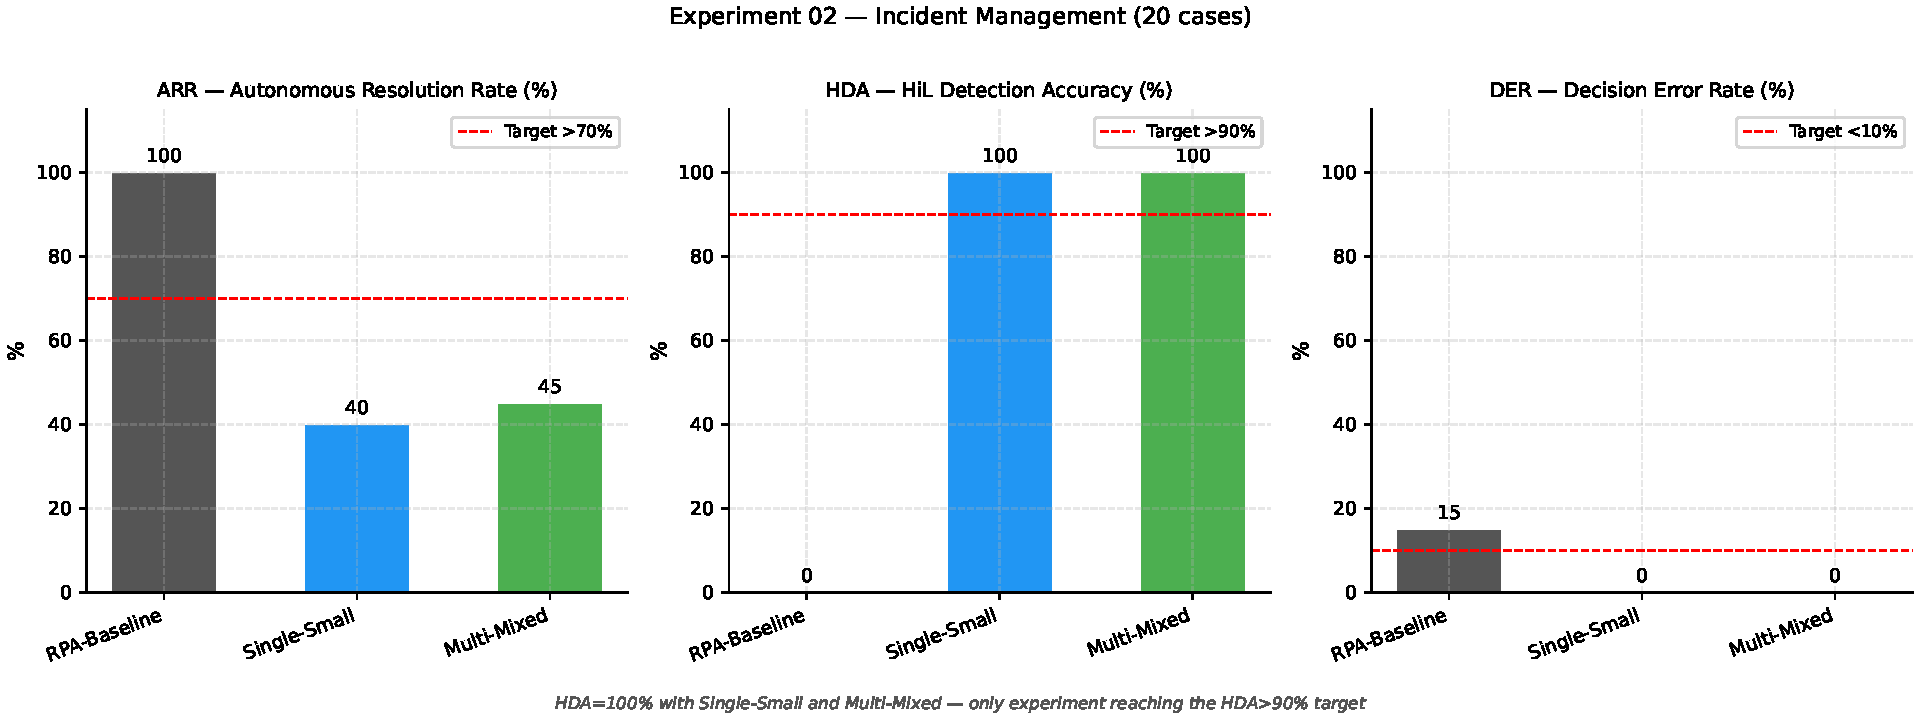
\includegraphics[width=\textwidth,height=0.42\textheight,keepaspectratio]{figura_inc1_metrics}
  \caption{ARR and HDA metrics for incident management (explicit binary
           signals). Single-Small and Multi-Mixed both reach HDA\,=\,100\%
           when signals are directly readable.}
  \label{fig:incidencias}
\end{figure}

\subsection{Validation on BPI Challenge~2019}
We sampled 50~cases from the BPI Challenge~2019
\citep{vandongen2019bpi}, stratified across three complexity levels,
maintaining the same distribution as the main experiment.
To ensure a fair comparison, the APIs were reparametrized with real
data from the dataset: financial thresholds were computed from actual
percentiles (P75\,=\,2,109\,EUR, max\,=\,8,833,459\,EUR) and compliance
rules were derived from the event log categories rather than artificial
assumptions.
The HiL escalation criterion is also objective and reproducible: a case
is labeled \texttt{requires\_hil=True} if it meets at least one of four
conditions, all derived directly from the event log: Consignment
category, Framework Order, amount exceeding 100,000\,EUR, or presence
of cancellation activities.
\begin{table}[H]
\centering
\caption{BPI Challenge~2019 vs.\ synthetic dataset comparison. The
         fragmentation patterns replicate on real data. Synthetic
         values for Single-Small-XL and Multi-Small report the mean
         over four replications.}
\label{tab:bpi}
\resizebox{\textwidth}{!}{%
\begin{tabular}{lcccccc}
\toprule
\textbf{Model} &
  \multicolumn{2}{c}{\textbf{ARR}} &
  \multicolumn{2}{c}{\textbf{HDA}} &
  \multicolumn{2}{c}{\textbf{DER}} \\
\cmidrule(lr){2-3}\cmidrule(lr){4-5}\cmidrule(lr){6-7}
& \textbf{BPI} & \textbf{Synthetic} & \textbf{BPI} & \textbf{Synthetic} &
  \textbf{BPI} & \textbf{Synthetic} \\
\midrule
RPA-Baseline & 100\% & 100\%                & 0.0\%  &  0.0\%               & 22\% & 34\% \\
Single-Small &  84\% &  76\%                & 45.5\% & 30.8\%               & 16\% & 22\% \\
Multi-Small  &  92\% &  79.5\%\,$\pm$\,7.1  &  9.1\% & 17.3\%\,$\pm$\,8.5  & 34\% & 27.5\% \\
Multi-Mixed  &  94\% &  99\%                & 18.2\% &  5.1\%               & 18\% & 27\% \\
\bottomrule
\end{tabular}%
}
\end{table}
Three main findings replicate on real data. First, the single agent
continues to detect risk better than the multi-agent system:
Single-Small achieves HDA\,=\,45.5\% vs.\ 9.1\% for Multi-Small.
The observed pattern is consistent with a context-fragmentation
explanation and was also present in the real event log of a
multinational company. Second, Multi-Small makes more decision errors
(DER\,=\,34\% vs.\ 16\% for Single-Small), reinforcing that
multi-agent architecture with small models not only detects risk less
reliably but also decides less accurately. Third, both Single-Small
and Multi-Small resolve a comparable share of cases autonomously on
BPI (84\% vs.\ 92\%), consistent with the compute equivalence pattern
observed in the synthetic experiment --- neither architecture produces
a decisive advantage with 8B models.

Single-Small detects more risk in BPI (45.5\%) than in the synthetic
dataset (30.8\%). The most plausible explanation is that BPI~2019
signals are more direct --- a Consignment order or an amount above
100,000\,EUR is straightforward to read. Detecting a GDPR violation
or an AESA certification issue requires domain-specific normative
knowledge that an 8B model does not reliably possess.

%%------------------------------------------------------------------------------
\section{Discussion}
\label{sec:discussion}

\subsection{Main Findings}

One pattern worth examining --- though the small number of HiL 
cases ($n=13$) limits any strong interpretation --- is that 
Multi-Mixed achieves HDA\,=\,5.1\%, while Single-Small reaches 
HDA\,=\,10.3\% on average (and 30.8\% in the first replication). 
One plausible explanation, consistent with the architecture, 
is the context fragmentation mechanism illustrated in 
Figure~\ref{fig:fragmentacion}. However, given the wide 
confidence intervals reported in Table~6, this should be 
treated as a hypothesis rather than a confirmed finding.

\begin{figure}[H]
\centering
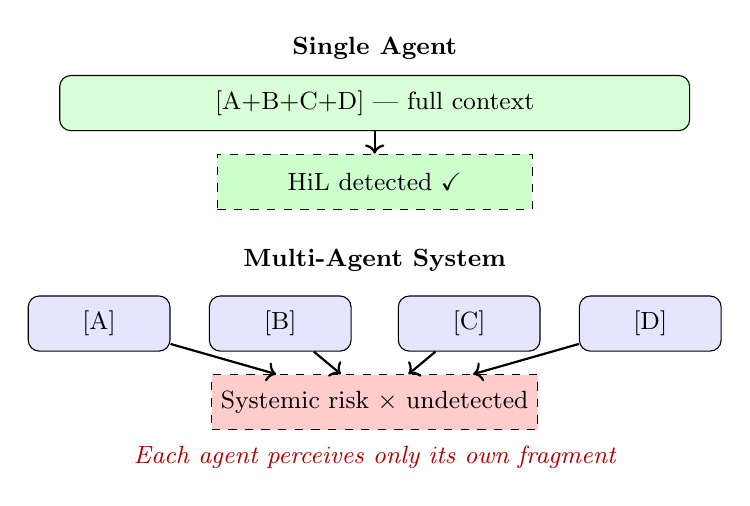
\begin{tikzpicture}[
  agent/.style={rectangle, draw, rounded corners, fill=blue!10,
                minimum width=1.8cm, minimum height=0.7cm, font=\small},
  risk/.style={rectangle, draw, dashed, fill=red!10,
               minimum width=1.8cm, minimum height=0.7cm, font=\small},
  arrow/.style={->, thick}
]
\node[font=\bfseries\small] at (0, 3.5) {Single Agent};
\node[agent, fill=green!15, minimum width=8cm] (single) at (0, 2.8)
  {[A+B+C+D] --- full context};
\node[risk, fill=green!20, minimum width=4cm] (detect) at (0, 1.8)
  {HiL detected \checkmark};
\draw[arrow] (single) -- (detect);
\node[font=\bfseries\small] at (0, 0.8) {Multi-Agent System};
\node[agent] (a1) at (-3.5, 0) {[A]};
\node[agent] (a2) at (-1.2, 0) {[B]};
\node[agent] (a3) at (1.2, 0) {[C]};
\node[agent] (a4) at (3.5, 0) {[D]};
\node[risk, fill=red!20, minimum width=4cm] (missed) at (0, -1.0)
  {Systemic risk $\times$ undetected};
\draw[arrow] (a1) -- (missed);
\draw[arrow] (a2) -- (missed);
\draw[arrow] (a3) -- (missed);
\draw[arrow] (a4) -- (missed);
\node[font=\itshape\small, text=red!70!black] at (0, -1.7)
  {Each agent perceives only its own fragment};
\end{tikzpicture}
\caption{Context fragmentation mechanism. The single agent integrates
         all risk factors into one decision; in the multi-agent
         architecture each agent perceives only its fragment and
         cross-cutting risk goes undetected.}
\label{fig:fragmentacion}
\end{figure}

The compute equivalence pattern is also clear: over four replications,
Single-Small-XL and Multi-Small converge to nearly identical ARR means
(79.0\% vs.\ 79.5\%), with overlapping standard errors. With 8B models,
neither expanding the context window nor adding specialized agents
produces a consistent advantage. The capacity threshold appears to lie
between 8B and 70B for this type of task \citep{Li2024moreagents}.

Model diversity is the highest-impact change in the experiment:
+19.2\,pp in ARR simply by replacing the 8B decision-maker with a 70B
model.

\subsection{Connection to Organizational Theories}


Three classical theories offer a lens for interpreting these 
patterns --- though the connections are interpretive rather 
than empirically derived from the data.

Simon's \emph{bounded rationality} \citep{simon1955rational} 
is perhaps the most relevant analogy. Each specialized agent 
acts rationally within its partial context, but the collective 
system may fail to detect risks requiring cross-cutting 
integration. The ablation data are consistent with this: 
removing Legal and Procurement drops HDA to 0\% (A3), while 
removing only Compliance raises it to 53.8\%. This pattern 
suggests that intermediation structure matters, though the 
small $n$ limits causal inference.

The ablation results are also consistent with Ricardo's comparative 
advantage \citep{ricardo1817}: Legal detects contractual risks better 
than any other agent, and Procurement handles supplier risks. The 
17.3\,pp of HDA lost when both are removed suggests specialization 
has value. The cost, however, is that no single agent holds the full 
risk picture --- a pattern Olson \citep{olson1965} would describe as 
a collective action problem, though we apply this analogy cautiously 
given the exploratory nature of the HDA data.

Finance's position in the DAG resembles what Granovetter 
\citep{granovetter1973} calls a weak tie: it bridges operational 
and regulatory decision-making. The RCD of Compliance ($-$23\,pp) 
is consistent with this --- removing it reduces fragmentation but 
raises DER to 74\%, an unacceptable trade-off in practice. These 
theoretical parallels are offered as interpretive scaffolding, 
not as empirically tested claims.

\subsection{Limitations}
\label{sec:limitations}

The most relevant limitation is that no configuration reached
HDA\,$>$\,90\%. The maximum in production-ready variants was 30.8\%.
The 10~undetected HiL cases correspond mostly to domain-specific
regulations (GDPR, AESA, CE certification) that the classifier's
generic features do not capture.

The DAG is sequential and allows no iteration: if one agent makes an
error, the subsequent agents cannot correct it. The 8B model is
unreliable across replications ($\sigma$\,=\,11.3\,pp), which makes
Single-Small results difficult to interpret reliably. On the
statistical side, 13~HiL cases are too few to draw strong conclusions
about HDA; the Bayes factor BF$_{10}$\,=\,0.41 indicates the evidence
is anecdotal. HDA-related analyses should be treated as exploratory
given the small number of positive cases, which limits the statistical
power of any between-variant comparison on this metric. Finally, the
APIs, while reparametrized with real BPI~2019 data, do not behave
identically to a real ERP or CRM system in production.
The 50~BPI cases were selected using domain-specific stratification
criteria to ensure coverage of all HiL signal types defined in the
taxonomy (Consignment, Framework Order, high-value transactions, and
cancellation activities). A post-hoc exploration of random sampling
from the full event log revealed that unconstrained sampling produces
a HiL distribution dominated by cancellation signals ($>$99\% of
positive cases), which confirms that procurement risk validation
requires deliberate stratification rather than generic random sampling.

\subsection{Ethical Considerations}

Three ethical issues should be addressed before any real-world
deployment.

The first is bias. LLMs can inherit implicit preferences from their
training data --- for example, favoring suppliers from certain countries
without anyone having explicitly programmed that behavior. This requires
periodic auditing of automated decisions.

The second is transparency. The system generates textual justifications
(SAT\,$>$\,3.5 in Multi-Mixed), but does not expose how it reached that
decision internally. In regulated environments that is not sufficient;
XAI techniques such as LIME or SHAP would need to be integrated over
the final decisions.

The third is accountability. With a maximum HDA of 30.8\%, a
significant share of risk cases are resolved without human oversight.
In real production, fixed escalation thresholds would be required ---
for example, any amount above 50,000\,EUR or any case flagged as GDPR
or AESA should always go to human review, regardless of the model's
decision.

%%------------------------------------------------------------------------------
\section{Conclusions and Future Work}
\label{sec:conclusions}

This work started from a concrete question: can a multi-agent system
resolve in seconds what procurement today takes days to process?
Technically, yes. What we did not expect is that adding more specialized
agents could actually worsen risk detection.

Multi-Mixed --- 8B auxiliaries, 70B decision-maker --- reaches
ARR\,=\,98.7\,\% with variability of $\pm$0.9\,pp, processes requests
in 1.74\,s, and carries an estimated cost of \$0.0065 per case. But
risk detection is the weak point: HDA\,=\,5.1\,\% in Multi-Mixed,
while Single-Small achieves HDA\,=\,10.3\,\% on average. These
figures are based on $n=13$ positive HiL cases and should be
read as preliminary evidence, not definitive results --- no
HDA comparison reaches statistical significance
(BF$_{10}$\,=\,0.41). Still, the pattern is consistent across
replications and warrants attention: a system can autonomously
resolve 98.7\,\% of cases and still miss the ones that matter most.

Architecture and information flow matter far more than the processing
capacity of each individual agent. With 8B models, neither expanding
the context window nor adding specialized agents produces a consistent
ARR advantage --- Single-Small-XL and Multi-Small converge to the same
mean over four independent runs (79.0\% vs.\ 79.5\%). Beyond ARR,
specialization introduces a trade-off with risk detection: specialists
become blind within their own silos, unable to pass along the context
that gives meaning to what they do.

The findings suggest that the path toward higher HDA likely does not
run through better models or more agents alone. One possible direction
is a role whose sole purpose is not to process invoices or review
regulations, but to examine the overall flow and identify the pieces
that do not fit together across agents --- a cross-process synthesizer:
Requester $\to$ Procurement $\to$ Finance $\to$ Synthesizer $\to$
Legal $\to$ Compliance, integrating the partial outputs before the
escalation decision and preserving specialization without succumbing to
the silos identified here. This hypothesis requires empirical validation
with more advanced architectures and additional domains.

Several lines of work remain open. The most immediate is extending the
Multi-Mixed-HiL-Clf classifier with domain-specific regulatory factors
(GDPR, AESA, CE certification) that are currently not captured. It also
makes sense to connect the system to real ERP/CRM APIs and evaluate
whether the signal explicitness gradient holds in other domains --- HR,
customer service, supply chain.

One final consideration: next-generation models \citep{OpenAI2023gpt4}
will likely shift the thresholds identified here (8B--70B). When that
happens, the trade-off analysis will remain relevant. Only the location
of the boundary will change.

Multi-agent architecture does not outperform the single agent by 
default. It does so when the underlying model has sufficient 
capacity to benefit from specialization --- and even then, 
the evidence here suggests it does not guarantee better 
systemic risk detection. Multi-Mixed reaches ARR\,=\,98.7\,\% 
but HDA\,=\,5.1\,\% across only $n=13$ positive cases, 
so this gap should be interpreted cautiously. What the data 
do support more robustly is that information flow between 
agents matters --- redesigning it is a more promising 
direction than simply adding models or agents.

%%------------------------------------------------------------------------------
\section*{Acknowledgments}

This work was carried out as part of a master's internship at
PROJENER.AI SL, Madrid. The author thanks Jesús Gil Ruiz (PROJENER.AI
SL) for his supervision during the internship, and Rafael Saucedo
Calzada (Universidad Alfonso X el Sabio, Campus Mare Nostrum) for his
academic guidance throughout the work.
%%------------------------------------------------------------------------------
%% NOTE: upload the .bib file with the name: references_multiagent.bib
\bibliographystyle{elsarticle-num}
\bibliography{references_multiagent}

%%------------------------------------------------------------------------------
\appendix
\section{Agent System Prompts}
\label{app:prompts}
\lstset{
  basicstyle=\ttfamily\footnotesize,
  breaklines=true,
  breakatwhitespace=false,
  breakindent=0pt,
  linewidth=\linewidth,
  columns=flexible
}

The prompts for all five agents are included below. The complete set
with additional parameters is available in the public repository.

\subsubsection*{Requester Agent}
\begin{lstlisting}[language={}, numbers=none]
role: "Request Manager"
goal: "Register and structure purchase requests."
backstory: "You are the first point of contact. You register requests
            and prepare them for the team."
\end{lstlisting}

\subsubsection*{Finance Agent}
\begin{lstlisting}[language={}, numbers=none]
role: "Finance Director"
goal: "Verify budget availability and validate the requested amount."
backstory: "You are responsible for budget control. You check the
            department's available budget and determine whether the
            requested amount is within approved limits."
\end{lstlisting}

\subsubsection*{Procurement Agent}
\begin{lstlisting}[language={}, numbers=none]
role: "Procurement Manager"
goal: "Validate the supplier and verify their approval status."
backstory: "You are a specialist in supplier management. You verify
            that the supplier is approved, has no conflict-of-interest
            alerts, and meets company requirements."
\end{lstlisting}

\subsubsection*{Legal Agent}
\begin{lstlisting}[language={}, numbers=none]
role: "Senior Legal Advisor"
goal: "Review contractual compliance and detect legal risks."
backstory: "You are familiar with GDPR, AESA, CE, and PRL regulations.
            You analyze risk clauses in contracts and issue a legal
            recommendation."
\end{lstlisting}

\subsubsection*{Compliance Agent}
\begin{lstlisting}[language={}, numbers=none]
role: "Compliance Director"
goal: "Verify regulatory compliance and escalate when risk exceeds
      established thresholds."
backstory: "You are the final decision-maker. You have authority to
            approve, reject, or escalate to the responsible human."
\end{lstlisting}

\section{Reproducibility Parameters}
\label{app:reproducibility}

\begin{itemize}
  \item Framework: CrewAI, Python~3.12, Windows~10, Jupyter~Lab
  \item Auxiliary LLM: \texttt{llama-3.1-8b-instant} via Groq~API
  \item Decision LLM (Mixed/Large): \texttt{llama-3.3-70b-versatile} via Groq~API
  \item Temperature: 0.0 (with the caveat documented in Sec.~\ref{sec:setup})
  \item Anti-rate-limit pause: 4--8~s between cases
  \item Code and datasets: \url{https://github.com/Edurne0781/multiagent-procurement-llm}
\end{itemize}

The BPI~Challenge~2019 is available at
DOI:~\texttt{10.4121/uuid:d06aff4b-79f0-45e6-8ec8-e19730c248f1}
(CC~BY~4.0).

\section{BPI Challenge~2019 Annotation Protocol}
\label{app:bpi_protocolo}

A case is labeled \texttt{requires\_hil=True} if it meets at least one
of the following criteria derived directly from the event log:
(a) category \texttt{Consignment}; (b) document type
\texttt{Framework order}; (c) amount exceeding 100,000\,EUR; or
(d) presence of cancellation activities (\texttt{Cancel Invoice
Receipt} or \texttt{Cancel Goods Receipt}).

\section{Inter-Annotator Kappa --- Risk Signal Taxonomy}
\label{app:kappa_matrix}

Taxonomy validation (EB, MX, IR, SS) was carried out with 2~human
annotators and 4~independent LLMs. $\kappa$\,=\,0.652 (range:
[0.477--0.878]). Disagreements concentrate at the MX/IR boundary. The
detailed pairwise annotator table is available in the repository.

\section{Justification Quality: LLM-as-Judge}
\label{app:sat}
The cost comparison in Figure~\ref{fig:coste} shows that Multi-Small
and Single-Small-XL share the exact same token budget (\$0.0045/case),
yet Single-Small-XL achieves an ARR 16\,pp higher. That gap is the
compute equivalence hypothesis expressed in numbers. The SAT scores
below reflect justification quality for the main variants.

\begin{table}[H]
\centering
\caption{LLM-as-Judge evaluation of justification quality (1--5 scale,
         $n=15$ cases). SAT\,=\,mean(Clarity, Completeness,
         Actionability). Target: SAT\,$>$\,3.5.}
\label{tab:sat}
\begin{tabular}{lcccc}
\toprule
\textbf{Variant} & \textbf{Clarity} & \textbf{Completeness} &
  \textbf{Actionability} & \textbf{SAT} \\
\midrule
RPA-Baseline & 3.67 & 3.20 & 2.40 & 3.09\,$\pm$\,0.67 \\
Single-Small & 4.20 & 3.60 & 4.00 & 3.93\,$\pm$\,0.69 \\
Multi-Small  & 4.07 & 3.86 & 4.14 & 4.02\,$\pm$\,0.55 \\
Multi-Mixed  & \textbf{4.27} & \textbf{4.53} & \textbf{4.27} & \textbf{4.36\,$\pm$\,0.27} \\
\bottomrule
\end{tabular}
\end{table}

The justification quality results are consistent with the ARR findings:
Multi-Mixed not only resolves more cases but also explains its decisions
more clearly. The actionability score of RPA-Baseline (2.40) reflects
its core limitation precisely --- it approves or rejects without giving
the recipient any useful context.

\section{Qualitative Error Analysis}
\label{app:errors}

\paragraph{Case C40 (GDPR + foreign cloud supplier).}
Multi-Mixed approves it: supplier is registered, budget is available.
Single-Small escalates it in replication~1 by detecting the combination
of foreign supplier and personal data. The GDPR risk is not captured as
an explicit factor in the mock APIs.

\paragraph{Case C43 (Conflict of interest + high amount).}
This case was correctly detected. Multi-Mixed-HiL-Clf escalates it:
the supplier has a conflict-of-interest alert and the amount exceeds
the board approval threshold. This is the profile the classifier
handles well: quantifiable, combined signals.

\section{Detailed AutoGen vs.\ CrewAI Comparison}
\label{app:autogen}

AutoGen~0.7.5 with default RoundRobin on the same 50~cases:
ARR\,=\,100\%, HDA\,=\,0\%, DER\,=\,76\%, PT\,=\,6.55\,s. Processing
time is nearly four times that of CrewAI (Multi-Mixed: 1.69\,s). These
results characterize default behavior, not the maximum achievable with
AutoGen. The relevant finding: HDA\,=\,0\% in both frameworks under
basic configuration, which supports the conclusion that the HiL
mechanism requires explicit design.

\section{Multi-Mixed-HiL-Clf Classifier Pseudocode}
\label{app:pseudocodigo}

\begin{lstlisting}[language=Python]
def hil_classifier(case):
    # Stage 1: Uncertainty Evaluator
    factors = extract_risk_factors(case)
    confidence = evaluate_confidence(factors)  # "high"|"low"
    if confidence == "low":
        return escalate_to_hil(case, summary=factors)
    # Stage 2: Senior Manager
    return senior_manager_decides(case, factors)
\end{lstlisting}




%%------------------------------------------------------------------------------
\section*{Data Availability Statement}
The BPI Challenge~2019 dataset ($n=251{,}734$) is publicly available
under CC~BY~4.0 at
DOI:~\texttt{10.4121/uuid:d06aff4b-79f0-45e6-8ec8-e19730c248f1}
\citep{vandongen2019bpi}. The synthetic dataset (50~cases), the five
secondary datasets (130~cases), the code, and the system prompts are
available at:
\url{https://github.com/Edurne0781/multiagent-procurement-llm}.
The repository will be archived on Zenodo with a permanent DOI prior
to publication.

\section*{Ethics Statement}
This work does not involve human subjects, personal data, or animal
experiments. The BPI Challenge~2019 contains anonymized industrial
logs (CC~BY~4.0). The inter-annotator validation involved voluntary
participation with no collection of personal data. No ethical approval
was required.

\section*{CRediT Author Contribution Statement}
\textbf{Edurne Martínez de Contrasta}: Conceptualization, Methodology,
Software, Formal analysis, Investigation, Data curation,
Writing -- original draft, Writing -- review \& editing, Visualization.

\section*{Declaration of Competing Interest}
The authors declare no known competing financial interests or personal
relationships that could have influenced the work reported in this paper.

\section*{Declaration of Generative AI and AI-Assisted Technologies}
During the preparation of this work, the author used generative AI
tools --- specifically Claude~Sonnet~4.6 (Anthropic) --- to assist
with writing tasks, grammatical revision, and text structuring. These
tools played no role in the experimental design, data generation,
statistical analysis, or interpretation of results. All content was
reviewed, edited, and validated by the author, who takes full
responsibility for the accuracy, integrity, and originality of the
manuscript. This declaration complies with Elsevier's policy on the
use of generative AI \citep{Elsevier2025ai}.

\end{document}